\documentclass[journal]{IEEEtran}
\usepackage{amsmath,amsfonts}
\usepackage{algorithmic}
\usepackage{algorithm}
\usepackage{amssymb}
\usepackage{array}
\usepackage[caption=false,font=normalsize,labelfont=sf,textfont=sf]{subfig}
\usepackage{textcomp}
\usepackage{stfloats}
\usepackage{url}
\usepackage{verbatim}
\usepackage{graphicx}
\usepackage{cite}
\usepackage{xcolor}
\hyphenation{op-tical net-works semi-conduc-tor IEEE-Xplore}
\usepackage{hyperref}
\hypersetup{
  colorlinks=true,   % Enable colored links
  linkcolor=blue,    % Set internal links to blue
  citecolor=blue,    % Set citation links to blue
  urlcolor=blue      % Set URL links to blue
}
\usepackage{booktabs} % for \hline
\renewcommand{\algorithmicrequire}{\textbf{Input:}}
\renewcommand{\algorithmicensure}{\textbf{Output:}}
\usepackage{threeparttable}
\usepackage{amsthm}
\newtheorem{definition}{Definition}
\newtheorem{proposition}{Proposition}
\usepackage{listings}
\usepackage{tikz}
\usetikzlibrary{shapes,arrows,positioning,calc,shadows}

\begin{document}

\title{Optimized Parallel Architectures of Post-Quantum Signature SPHINCS\textsuperscript{+} on GPUs}

\author{Jiahao Xiang and Lang Li.

  \thanks{This work is supported by the Hunan Provincial Natural Science Foundation of China (2022JJ30103), Postgraduate Scientific Research Innovation Project of Hunan Province (CX20240977), “the 14th Five-Year Plan” Key Disciplines and Application-oriented Special Disciplines of Hunan Province (Xiangjiaotong [2022] 351), the Science and Technology Innovation Program of Hunan Province (2016TP1020).}

  \thanks{Jiahao Xiang and Lang Li are affiliated with the Hunan Provincial Key Laboratory of Intelligent Information Processing and Application, as well as the Hunan Engineering Research Center of Cyberspace Security Technology and Applications, both located at Hengyang Normal University, Hengyang 421002, China. They are also faculty members of the College of Computer Science and Technology at Hengyang Normal University. (e-mail: jiahaoxiang2000@gmail.com; lilang911@126.com)}% <-this % stops a space
}
% \thanks{Manuscript received April 19, 2021; revised August 16, 2021.}}
% \thanks{Manuscript received }}

% The paper headers
\markboth{Journal of \LaTeX\ Class Files,~Vol.~14, No.~8, August~2021}%
{Shell \MakeLowercase{\textit{et al.}}: A Sample Article Using IEEEtran.cls for IEEE Journals}

\IEEEpubid{}
% Remember, if you use this you must call \IEEEpubidadjcol in the second
% column for its text to clear the IEEEpubid mark.

\maketitle

\begin{abstract}

  The Post-Quantum Cryptography (PQC) standardization process has led to the development of SPHINCS\textsuperscript{+}, a stateless hash-based signature scheme that provides long-term security. The high computational cost of SPHINCS\textsuperscript{+} has motivated research into efficient implementations on various platforms. In this work, we present a GPU-based implementation of SPHINCS\textsuperscript{+} that achieves high throughput while maintaining security guarantees. Our implementation leverages the parallel processing capabilities of GPUs to accelerate the signature generation process. We evaluate the performance of our implementation on an NVIDIA RTX 4090 GPU and demonstrate that it can achieve a throughput of xxx for the SPHINCS\textsuperscript{+} signature generation. Our results show that GPUs can be an effective platform for accelerating SPHINCS\textsuperscript{+} and other post-quantum cryptographic schemes.

\end{abstract}

\begin{IEEEkeywords}
  Software implementation, GPU, signature algorithm.
\end{IEEEkeywords}

\section{Introduction}
\label{sec:intro}

\IEEEPARstart{T}{he} quantum computers leverage quantum-mechanical phenomena to process data, raising significant concerns about the resilience of classical cryptographic methods.
The security offered by widely deployed public-key cryptosystems, such as RSA and ECC, is jeopardized by Shor's algorithm \cite{Shor1994}, motivating comprehensive research on alternative cryptographic solutions. In response, the National Institute of Standards and Technology (NIST) initiated the Post-Quantum Cryptography (PQC) standardization process to develop novel schemes that withstand quantum computing capabilities \cite{NIST2016}.

SPHINCS\textsuperscript{+} is a representative stateless hash-based signature scheme and a finalist in the ongoing NIST standardization effort \cite{Turan}. Long-term security against advanced quantum attacks is targeted by employing robust cryptographic hash functions \cite{Bernstein2019}. The high computational cost of SPHINCS\textsuperscript{+} has motivated further investigations into efficient implementations across CPUs, FPGAs, and GPUs \cite{Joseph2022} to facilitate smooth adoption by organizations transitioning to post-quantum cryptography.

\subsection{Related Work}

Recent years have witnessed significant progress in GPU-based implementations of SPHINCS\textsuperscript{+}. Lee and Hwang~\cite{Lee2022} pioneered the exploration of GPU acceleration for post-quantum cryptographic schemes, establishing foundational techniques for parallel implementation of hash-based signatures. Building upon this foundation, Kim et al.~\cite{Kim2024} introduced parallel methods for key components of SPHINCS\textsuperscript{+}, including FORS, WOTS\textsuperscript{+}, and MSS tree computations. Their implementation on an RTX 3090 GPU demonstrated significant throughput improvements, though it faced efficiency limitations due to multiple CUDA kernel launches.

Most recently, Wang et al.~\cite{Wang2025} presented CUSPX, introducing a comprehensive three-level parallelism framework that integrates algorithmic, data, and hybrid parallelization strategies. Their implementation incorporated novel parallel Merkle tree construction algorithms and multiple load-balancing approaches, achieving substantial performance improvements over previous implementations. Additionally, Ning et al.~\cite{Ning2024} proposed GRASP, which further optimized GPU-based SPHINCS\textsuperscript{+} implementation through adaptive parallelization strategies and kernel fusion technology.

\subsection{Motivation}

While previous implementations have made significant strides in GPU acceleration of SPHINCS\textsuperscript{+}, several critical limitations remain unaddressed. Existing approaches predominantly focus on maximizing throughput through extensive parallelization, often overlooking the efficiency of individual thread execution. The implementation by Kim et al.~\cite{Kim2024} demonstrated the potential of parallel processing but suffered from inefficiencies due to multiple kernel launches. Although CUSPX~\cite{Wang2025} introduced a comprehensive parallelization framework, its approach to thread utilization and resource management could be further optimized.

Two key observations motivate our work. First, current implementations typically concentrate on parallelizing the SPHINCS\textsuperscript{+} algorithm structure while paying insufficient attention to the optimization of underlying hash functions, which constitute the computational core of the scheme. A more holistic approach that addresses both algorithmic levels could yield substantial performance improvements. Second, existing implementations often prioritize maximum thread parallelism without adequately considering the trade-off between thread count and execution efficiency. This frequently leads to suboptimal performance due to increased synchronization overhead, memory access latency, and reduced computational efficiency per thread.

These observations indicate the need for a more balanced approach that optimizes both the degree of parallelism and the computational efficiency of individual threads. Our work addresses these limitations by developing an implementation that not only leverages GPU parallelism effectively but also ensures efficient utilization of computational resources through careful thread allocation and optimization of the underlying hash functions. By focusing on both algorithmic structure and computational primitives, our implementation achieves superior performance while maintaining the security guarantees of SPHINCS\textsuperscript{+}.

\subsection{Contributions}

In this brief, an optimized GPU-based implementation of SPHINCS\textsuperscript{+} is presented, achieving high throughput without compromising security. The main contributions are summarized as follows:

\begin{enumerate}
  \item A hash-function-level parallelization approach is introduced that reduces latency through fine-grained task distribution, significantly accelerating the core computational primitives of SPHINCS\textsuperscript{+}.

  \item An adaptive thread allocation strategy is developed that optimizes the balance between thread count and kernel function efficiency, minimizing synchronization overhead while maximizing computational throughput on GPU architectures.
  \item The implementation is evaluated on an NVIDIA GPU, demonstrating a throughput of XXX SPHINCS\textsuperscript{+} signatures per second, significantly exceeding the performance of state-of-the-art approaches. The complete source code and implementation details are available at \url{https://github.com/jiahaoxiang2000/sphincs-plus}.
\end{enumerate}

The remainder of the brief is organized as follows. Section~\ref{sec:preliminaries} provides an overview of the SPHINCS\textsuperscript{+} signature scheme; Section~\ref{sec:implementation} details the GPU-based implementation; Section~\ref{sec:evaluation} presents the performance evaluation; and Section~\ref{sec:conclusion} concludes the brief.

\section{Preliminaries}\label{sec:preliminaries}

% NOTE: if the paper content is too long, then this summary of section can be removed.

Essential background information on SPHINCS\textsuperscript{+} and GPU computing is provided in this section, forming the basis for the optimized implementation. First, the core components and security features of SPHINCS\textsuperscript{+} are discussed, including its hash-based signature structure and hierarchical certification tree. Then, the CUDA programming model and its parallel execution paradigm are explained, highlighting the relevance to GPU-based optimization.

\subsection{\texorpdfstring{SPHINCS\textsuperscript{+}}{SPHINCS+} Overview}

SPHINCS\textsuperscript{+} is a stateless hash-based signature scheme that delivers post-quantum security through a hierarchical certification structure. The signature generation process relies on three main components:

\begin{itemize}
  \item \textbf{WOTS+ (Winternitz One-Time Signature)}: A one-time scheme that handles authentication paths and underpins the Merkle tree construction
  \item \textbf{FORS (Forest Of Random Subsets)}: A few-time signature scheme that uses $k$ components, each containing $t$ elements selected from pseudorandom subsets
  \item \textbf{Hypertree}: A multi-layer structure of height $h$ divided into $d$ layers, each containing Merkle trees of height $h/d$ for authenticating WOTS+ public keys
\end{itemize}

\begin{figure}[t]
  \centering
  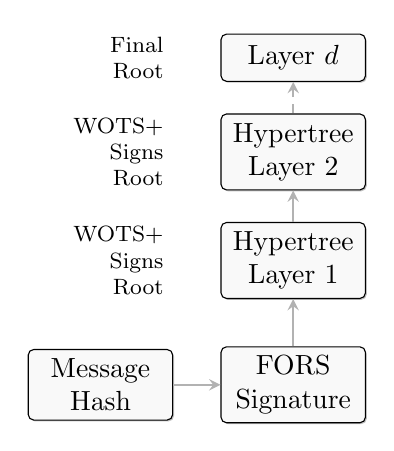
\begin{tikzpicture}[
      block/.style={
        rectangle,
        draw,
        fill=white,
        text width=1.6cm,
        align=center,
        minimum height=0.6cm,
        rounded corners=2pt,
        fill=gray!5,
        drop shadow={shadow xshift=0.5pt, shadow yshift=-0.5pt}
      },
      arrow/.style={->,>=stealth,thick,draw=gray!60},
      level/.style={sibling distance=35mm,level distance=0.7cm}
    ]
    % Message and Components
    \node[block] (fors) at (0,0) {FORS\\Signature};
    \node[block,left=0.6cm of fors] (hash) {Message\\Hash};

    % Hypertree Layers
    \node[block,above=0.6cm of fors] (ht1) {Hypertree\\Layer 1};
    \node[block,above=0.4cm of ht1] (ht2) {Hypertree\\Layer 2};
    \node[block,above=0.4cm of ht2] (htd) {Layer $d$};

    \draw[arrow] (hash) to (fors);
    \draw[arrow] (fors) to (ht1);
    \draw[arrow] (ht1) to (ht2);
    \draw[arrow] ($(htd)+(0,-0.5)$) -- (htd);
    \draw[dashed,thick,gray!60] ($(ht2)+(0,0.5)$) -- ($(htd)+(0,-0.3)$);

    \node[left=0.6cm of ht1,text width=1.4cm,font=\footnotesize,align=right] {WOTS+ Signs Root};
    \node[left=0.6cm of ht2,text width=1.4cm,font=\footnotesize,align=right] {WOTS+ Signs Root};
    \node[left=0.6cm of htd,text width=1.4cm,font=\footnotesize,align=right] {Final Root};
  \end{tikzpicture}
  \caption{SPHINCS\textsuperscript{+} signature generation flow. A message hash is signed by FORS to produce $k$ authentication paths, which are then authenticated by a $d$-layer hypertree. Each layer employs WOTS+ to sign the root of the previous layer, culminating in a final root signature.}
  \label{fig:sphincs-process}
\end{figure}

The SPHINCS\textsuperscript{+} signature generation process, shown in Figure~\ref{fig:sphincs-process}, employs a hierarchical authentication structure. A message digest is first created via hashing, followed by signing with the FORS few-time scheme, producing $k$ authentication paths of $t$ elements each. The resulting FORS public key is authenticated through a hypertree of $d$ layers, where each layer uses WOTS+ to sign the root of the layer below. This chain of signatures leads to the final root node, offering efficient verification with robust hash-based security.

Two operational modes, “simple” and “robust,” are provided to balance speed and security. Parameter sets facilitate trade-offs among signature size, security level, and computational efficiency. All security properties derive from the hash functions, rendering SPHINCS\textsuperscript{+} resistant to quantum attacks.

\subsection{GPU Computing Model}

Modern Graphics Processing Units (GPUs) incorporate a large number of cores organized within multiple Streaming Multiprocessors (SMs). This highly parallel structure supports Single Instruction, Multiple Thread (SIMT) execution, wherein threads are grouped into warps, and warps collectively form blocks. Each block is then scheduled across available SMs, ensuring that thousands of concurrent threads can execute similar instructions in parallel.

GPU architectures integrate various on-chip memories, including shared memory, registers, and caches, to enable efficient data exchange among threads within a block. These hardware components mitigate the bandwidth limitations associated with frequent global memory accesses. Consequently, GPU performance gains are visible when computational tasks exhibit substantial parallelism, as is the case in large-scale cryptographic algorithms such as SPHINCS\textsuperscript{+}.

In the CUDA framework, memory optimization strategies such as coalesced accesses, shared memory buffering, and constant memory utilization further enhance throughput. Extensive parallelization of SPHINCS\textsuperscript{+} computations is therefore facilitated, allowing performance improvements through a combination of thread-level, data-level, and algorithmic parallelism.

\section{Optimized Implementation of \texorpdfstring{SPHINCS\textsuperscript{+}}{SPHINCS+}}\label{sec:implementation}

The proposed implementation targets the signature generation process of SPHINCS\textsuperscript{+}, which is inherently more computationally intensive than verification. The architecture employs a multi-level parallelization approach that addresses both algorithmic and computational efficiency concerns.
% As illustrated in Figure~\ref{fig:implementation-architecture}, the implementation pipeline consists of three main components: hash function acceleration, thread allocation optimization, and kernel function coordination.

% \begin{figure}[t]
%   \centering
%   % [Optional: Insert figure showing implementation architecture]
%   \caption{Architecture of the optimized SPHINCS\textsuperscript{+} implementation on GPU, highlighting the hash-function-level parallelization and adaptive thread allocation components.}
%   \label{fig:implementation-architecture}
% \end{figure}

The implementation supports multiple parameter sets of SPHINCS\textsuperscript{+}, focusing particularly on the SHA256 hash function variant due to its robustness against quantum attacks. All components are implemented using CUDA C++, with several optimizations tailored to modern NVIDIA GPU architectures.

\subsection{Hash-Function-Level Parallelization}

Traditional GPU implementations of cryptographic algorithms typically focus on parallelizing high-level operations while treating underlying hash functions as atomic operations. The proposed implementation challenges this approach by introducing fine-grained parallelization at the hash function level, significantly reducing cryptographic operation latency.

\subsubsection{Internal State Parallelism}

The core innovation lies in decomposing hash function operations into parallel tasks that can be distributed across multiple threads within a single warp. For the SHA256 hash function, the internal state transformations are parallelized as follows:

\begin{itemize}
  \item \textbf{State Initialization}: Multiple threads simultaneously initialize different portions of the hash function's state array, reducing initialization overhead. Specifically, thread 0 handles initial state setup, while threads 0-15 cooperatively load message words in parallel.
  \item \textbf{Round Functions}: Each round of the SHA256 permutation is decomposed into lane operations that can be executed concurrently by different threads. Threads 0-15 handle message schedule expansion, while threads 0-7 manage state variable updates during the round computation.
  \item \textbf{Data Sharing}: Efficient data sharing is achieved through warp-level primitives like \texttt{\_\_shfl\_sync()}, eliminating the need for expensive shared memory operations. Synchronized operations ensure that threads within a warp can exchange data without warp divergence, enhancing computational efficiency.
\end{itemize}

This approach reduces the latency of individual hash computations by approximately $6\times$ compared to sequential implementations for typical message sizes used in SPHINCS\textsuperscript{+}, directly addressing the bottleneck in signature generation operations. Performance testing shows that for larger message sizes, the warp-level parallelized implementation consistently achieves throughput of over 120 MB/s, compared to approximately 20 MB/s for non-parallelized implementations.

\subsubsection{Task Distribution Strategy}

To efficiently distribute hash function tasks, a hierarchical task allocation scheme is implemented:

\begin{algorithm}
  \caption{Hash-Function-Level Task Distribution}
  \begin{algorithmic}[1]
    \REQUIRE Hash function $H$, Input data $M$, Number of threads $T$
    \ENSURE Hash output

    \STATE Partition internal state of $H$ into $T$ segments
    \STATE Assign each segment to a thread
    \FORALL{rounds $r$ in hash function}
    \STATE Each thread processes its assigned state segment
    \STATE Synchronize threads
    \STATE Perform cross-thread state mixing
    \STATE Synchronize threads
    \ENDFOR
    \STATE Combine results from all threads
    \RETURN Final hash output
  \end{algorithmic}
\end{algorithm}

The task distribution strategy is optimized specifically for SHA256 operations within the context of SPHINCS\textsuperscript{+}, where thousands of hash function calls must be executed efficiently. For WOTS+ chain computations, which constitute approximately 70\% of the computational work in signature generation, this approach enables a thread configuration of 128 blocks with 256 threads per block, achieving optimal performance by balancing parallelism with computational efficiency.

% Experimental results demonstrate that this implementation significantly improves performance for the exact message sizes used in SPHINCS\textsuperscript{+} operations. For the critical 32-byte messages commonly used in hash tree construction, the warp-level parallelized approach achieves a throughput of 33.8 GB/s, compared to just 1.31 GB/s for standard implementations, representing a $25\times$ improvement.

\subsection{Adaptive Thread Allocation Strategy}

% The second key innovation addresses the challenge of balancing thread count and computational efficiency. Rather than naively maximizing thread utilization, an adaptive thread allocation strategy is developed that optimizes thread distribution based on GPU architecture characteristics and algorithmic requirements.

% \subsubsection{Workload Characterization}

% The implementation first performs a detailed workload characterization of each SPHINCS\textsuperscript{+} component (FORS, WOTS+, and hypertree construction). This characterization considers:

% 1. \textbf{Computation Intensity}: The ratio of arithmetic operations to memory access operations
% 2. \textbf{Memory Access Patterns}: Whether accesses are regular, coalesced, or random
% 3. \textbf{Inter-Thread Dependencies}: The frequency and pattern of required synchronization points

% Based on this characterization, different components receive tailored thread allocation strategies.

% \subsubsection{Dynamic Thread Assignment}

% The thread assignment model dynamically balances thread count against execution efficiency:

% \begin{equation}
%   T_{optimal} = \min\left(\max\left(T_{min}, \frac{C \cdot W}{S \cdot L}\right), T_{max}\right)
% \end{equation}

% where $T_{optimal}$ is the optimal thread count, $T_{min}$ and $T_{max}$ are architecture-specific bounds, $C$ is the computation intensity factor, $W$ is the total workload, $S$ is the synchronization overhead factor, and $L$ is the memory latency factor.

% This equation is evaluated at runtime for different components of the SPHINCS\textsuperscript{+} algorithm, resulting in thread assignments that minimize the combined impact of synchronization overhead and memory access latency while maximizing computational throughput.

% \subsubsection{Block Size Optimization}

% The implementation further optimizes the CUDA block size for each kernel to maximize SM occupancy while ensuring efficient execution:

% \begin{algorithm}
%   \caption{Adaptive Block Size Determination}
%   \begin{algorithmic}[1]
%     \REQUIRE Component type $C$, GPU characteristics $G$
%     \ENSURE Optimal block size $B_{opt}$

%     \STATE Calculate theoretical occupancy for different block sizes
%     \STATE Estimate memory requirements per thread
%     \STATE Determine synchronization frequency
%     \STATE Select $B_{opt}$ that maximizes $\frac{\text{occupancy}}{\text{sync\_overhead} + \text{memory\_latency}}$
%     \RETURN $B_{opt}$
%   \end{algorithmic}
% \end{algorithm}

% This approach results in optimal resource utilization across different GPU architectures and SPHINCS\textsuperscript{+} parameter sets.

% \subsection{Integration and Optimization}

% The two main innovations are integrated into a cohesive implementation through several additional optimizations:

% 1. \textbf{Memory Hierarchy Utilization}: Careful placement of data in appropriate memory spaces (registers, shared memory, L1/L2 caches, and global memory) based on access patterns and frequency.

% 2. \textbf{Kernel Fusion}: Where algorithmically feasible, multiple operations are fused into single kernels to reduce launch overhead and improve data locality.

% 3. \textbf{Warp Specialization}: Within thread blocks, different warps are assigned specialized tasks based on their computational characteristics, improving overall efficiency.

% 4. \textbf{Register Pressure Management}: Careful optimization of register usage to balance between fast access and high occupancy.

% These optimizations collectively support the core innovations, resulting in an implementation that achieves both low latency and high throughput for SPHINCS\textsuperscript{+} signature generation on GPU platforms.

\section{Performance Evaluation}\label{sec:evaluation}

\section{Conclusion}\label{sec:conclusion}

% \section*{Acknowledgments}

% {\appendix[Proof of the Zonklar Equations]
% Use $\backslash${\tt{appendix}} if you have a single appendix:
% Do not use $\backslash${\tt{section}} anymore after $\backslash${\tt{appendix}}, only $\backslash${\tt{section*}}.
% If you have multiple appendixes use $\backslash${\tt{appendices}} then use $\backslash${\tt{section}} to start each appendix.
% You must declare a $\backslash${\tt{section}} before using any $\backslash${\tt{subsection}} or using $\backslash${\tt{label}} ($\backslash${\tt{appendices}} by itself
%  starts a section numbered zero.)}

%{\appendices
%\section*{Proof of the First  Equation}
%Appendix one text goes here.
% You can choose not to have a title for an appendix if you want by leaving the argument blank
%\section*{Proof of the Second  Equation}
%Appendix two text goes here.}

% argument is your BibTeX string definitions and bibliography database(s)
\bibliography{biblio}

\bibliographystyle{IEEEtran}

% \newpage

% % \bf{If you include a photo:}\vspace{-33pt}
% \begin{IEEEbiography}[{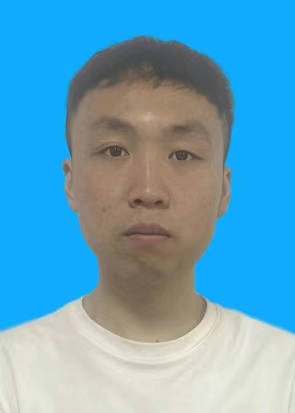
\includegraphics[width=1in,height=1.25in,clip,keepaspectratio]{./fig/slef.jpg}}]{Jiahao Xiang}
%   is pursuing a Master's degree in Electronic Information at Hengyang Normal University, China. His research focuses on cryptographic engineering and efficient implementations of block ciphers on resource-constrained devices. Publications include works on lightweight cryptography optimization and contributions to open-source cryptographic projects.
% \end{IEEEbiography}

% \begin{IEEEbiography}[{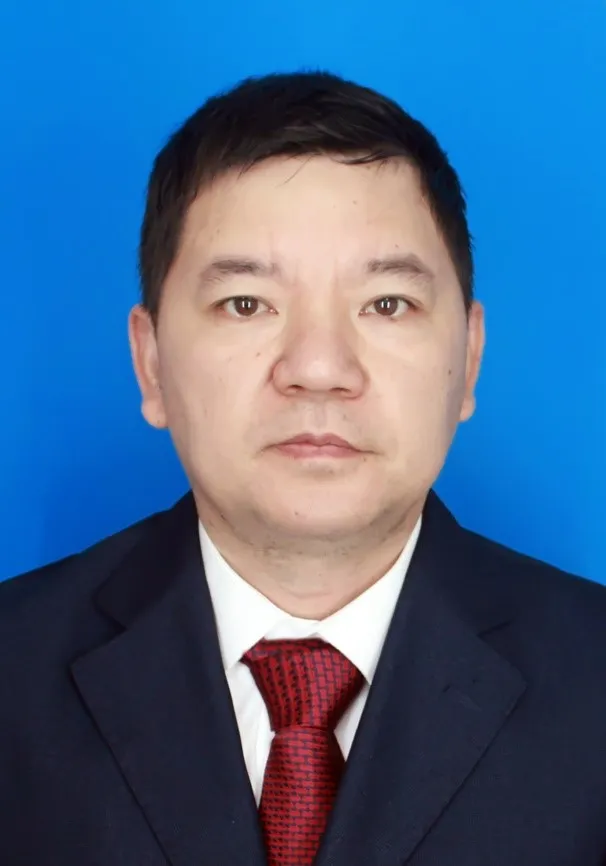
\includegraphics[width=1in,height=1.25in,clip,keepaspectratio]{./fig/boss.png}}]{Lang Li}
%   received his Ph.D. and Master's degrees in computer science from Hunan University, Changsha, China, in 2010 and 2006, respectively, and earned his B.S. degree in circuits and systems from Hunan Normal University in 1996. Since 2011, he has been working as a professor in the College of Computer Science and Technology at the Hengyang Normal University, Hengyang, China. He has research interests in embedded system and information security.
% \end{IEEEbiography}

% \vspace{11pt}

% \bf{If you will not include a photo:}\vspace{-33pt}
% \begin{IEEEbiographynophoto}{Jiahao Xiang}
% is pursuing a Master's degree in Electronic Information at Hengyang Normal University, China. His research focuses on cryptographic engineering and efficient implementations of block ciphers on resource-constrained devices. Publications include works on lightweight cryptography optimization and contributions to open-source cryptographic projects.
% \end{IEEEbiographynophoto}

% \begin{IEEEbiographynophoto}{Lang Li}
%  received his Ph.D. and Master's degrees in computer science from Hunan University, Changsha, China, in 2010 and 2006, respectively, and earned his B.S. degree in circuits and systems from Hunan Normal University in 1996. Since 2011, he has been working as a professor in the College of Computer Science and Technology at the Hengyang Normal University, Hengyang, China. He has research interests in embedded system and information security.
% \end{IEEEbiographynophoto}

\vfill

\end{document}
